\documentclass[tikz]{standalone}
\usepackage{amsmath}
\usepackage{tikz}

\begin{document}

\begin{figure}[h]
\begin{center}
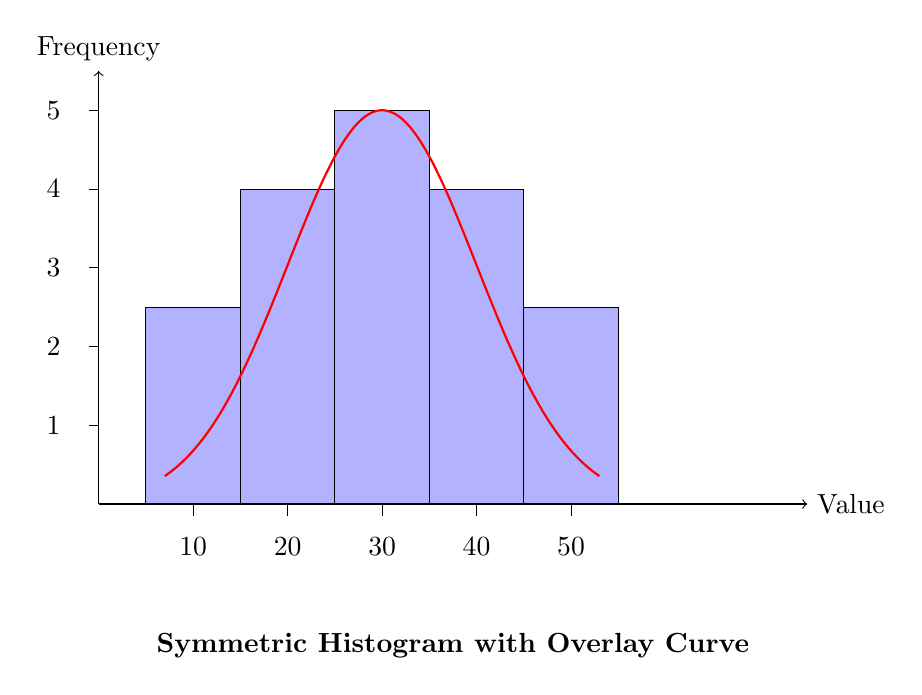
\begin{tikzpicture}[xscale=1.2, yscale=1]
  \draw[->] (0,0) -- (7.5,0) node[right] {Value};
  \draw[->] (0,0) -- (0,5.5) node[above] {Frequency};
  \filldraw[fill=blue!30] (0.5,0) rectangle (1.5,2.5);
  \filldraw[fill=blue!30] (1.5,0) rectangle (2.5,4);
  \filldraw[fill=blue!30] (2.5,0) rectangle (3.5,5);
  \filldraw[fill=blue!30] (3.5,0) rectangle (4.5,4);
  \filldraw[fill=blue!30] (4.5,0) rectangle (5.5,2.5);
  \foreach \x/\label in {1/10, 2/20, 3/30, 4/40, 5/50} {
    \draw (\x,0) -- (\x,-0.15);
    \node[below] at (\x,-0.3) {\label};
  }
  \foreach \y in {1,...,5} {
    \draw (0,\y) -- (-0.1,\y);
    \node[left] at (-0.3,\y) {\y};
  }
  \draw[thick, red, smooth, samples=100, domain=0.7:5.3]
    plot (\x, {5*exp(-0.5*(\x - 3)^2)});
  \node[font=\bfseries] at (3.75,-1.8) {Symmetric Histogram with Overlay Curve};
\end{tikzpicture}
\end{center}
\caption{An illustration of a histogram which has a symmetric probability distribution.}
\end{figure}

\end{document}